% Created 2020-06-30 Tue 07:07
% Intended LaTeX compiler: pdflatex
\documentclass[11pt]{article}
\usepackage[utf8]{inputenc}
\usepackage[T1]{fontenc}
\usepackage{graphicx}
\usepackage{grffile}
\usepackage{longtable}
\usepackage{wrapfig}
\usepackage{rotating}
\usepackage[normalem]{ulem}
\usepackage{amsmath}
\usepackage{textcomp}
\usepackage{amssymb}
\usepackage{capt-of}
\usepackage{hyperref}
\usepackage{color}
\usepackage{listings}
\usepackage[table,xcdraw]{xcolor}
\usepackage{listings}

% src: http://texdoc.net/texmf-dist/doc/latex/listings/listings.pdf
\lstdefinestyle{customc}{
  belowcaptionskip=1\baselineskip,
  breaklines=true,
  %frame=L,%lines, whole
  xleftmargin=\parindent,
  language=C,
  showstringspaces=false,
  basicstyle=\scriptsize\ttfamily,
  keywordstyle=\bfseries\color{green!40!black},
  commentstyle=\itshape\color{purple!40!black},
  identifierstyle=\color{blue},
  stringstyle=\color{orange},
  numberstyle={\tiny},
  numbers=left,
  numberblanklines=false,
  stepnumber=5,
  backgroundcolor=\color{yellow!10}, 
  frame=tlb
}

\lstdefinestyle{customasm}{
  belowcaptionskip=1\baselineskip,
  frame=L,
  xleftmargin=\parindent,
  language=[x86masm]Assembler,
  basicstyle=\footnotesize\ttfamily,
  commentstyle=\itshape\color{purple!40!black},
}

\lstset{escapechar=@,style=customc}

\author{José Miguel Alves Pires\thanks{a50178@alunos.uminho.pt}}
\date{\textit{<2020-06-30 Tue>}}
\title{cheatsheet}
\hypersetup{
 pdfauthor={José Miguel Alves Pires},
 pdftitle={cheatsheet},
 pdfkeywords={},
 pdfsubject={},
 pdfcreator={Emacs 26.3 (Org mode 9.3.6)}, 
 pdflang={English}}
\begin{document}

\maketitle
\tableofcontents


\section{Modular design\hfill{}\textsc{Important}}
\label{sec:org400fc2f}
Modular design is useful to separate logical units inside the \LaTeX{} environment.
\begin{itemize}
\item \texttt{dissertation.tex}: main document that defines all the formatting and includes
all the relevant \texttt{.tex} documents
\item \texttt{./sty}: contains the stylesheets for the document, such as:
\begin{itemize}
\item \texttt{dissertation-xelatex.sty}: stylesheet for the main document
\item \texttt{listing.sty}: stylesheet for the listings to be formatted and presented
\end{itemize}
\item \texttt{./sec}: contains secondary files, like images, PDFs, acronyms and symbols
\item \texttt{./bib}: contains the bibliography database
\item \texttt{./listing}: contains the listings (code) to be displayed
\item \texttt{./font}: contains the fonts to be used
\item \texttt{./tex}: contains the \texttt{.tex} documents to be inputted, subdivided in:
\begin{itemize}
\item \texttt{Pre\_Chap}: Pre chapters (not used here)
\item \texttt{Chap}: chapters
\item \texttt{Append}: appendices
\end{itemize}
\end{itemize}

Regarding \texttt{.tex} documents, they can be included as follows (the extension
\texttt{.tex} is implicit):
\begin{itemize}
\item \texttt{\textbackslash{}input\{path/to/file\}}: inputs the file as is (\textsubscript{recommended}\_)
\item \texttt{\textbackslash{}include\{path/to/file\}}: inputs the file and adds an extra blank page at the
end.
\end{itemize}

\section{Styling guides\hfill{}\textsc{Important}}
\label{sec:orga642a07}
\begin{enumerate}
\item Don't use \texttt{\textbackslash{}newpage}, \texttt{\textbackslash{}clearpage}, or any other section break command. This
is done natively by the \TeX{} engine; it should be done last and only if REALLY
required
\item To separate paragraphs use one blank line; any additional blank lines MUST BE
AVOIDED anywhere in the document. If you want to separate anything visually,
use a comment \texttt{\%}.
\begin{itemize}
\item Example:
\lstset{language=[LaTeX]TeX,label= ,caption= ,captionpos=b,numbers=none}
\begin{lstlisting}
%
\section{Product concept}%
\label{sec:product-concept}
\section{Product concept}%
\label{sec:orge7b0dc6}
The envisioned product consists of a remote controlled car used to assist
exploration and maintenance domains, hereby, denominated as Radio Frequency
Camera Assisted Rover (RFCAR). To satisfy such requirements, the vehicle must
contain a remotely operated camera that provides a live video feed to the user.
Additionally, the vehicle must include an odometric system that assists the
driving and avoids unintentional collisions when remote control is compromised, e.g., when connection is lost.
The vehicle provides means for exploration and conditions assessment in critical
or unaccessible areas to human operators, such as fluid pipelines and other hazardous locations.
%
%%% Local Variables:
%%% mode: latex
%%% TeX-master: "../Phase1"
%%% End:

%
\section{Foreseen specifications}%
\label{sec:fores-spec}
\section{Foreseen product specifications}
\label{sec:org31f7574}
The foreseen product specifications are listed as topics below (sketch).

\subsection{Autonomy}
\label{sec:org7364ba5}
The vehicle is operated off-the-grid, thus, a portable power source must be included. The autonomy referes to the time interval between battery fully charged and safely discharged and should be observed for the following scenarios:
\begin{itemize}
\item No load;
\item Vehicle operating at maximum speed;
\item Vehicle operating at minimum speed.
\end{itemize}
\subsection{Velocity}
\label{sec:org08718bc}
The velocity the car achieves is determined by the voltage of the motors, allowing to operate the car at the desired velocity simply varying the dutycicle of the control signal to the motors. The maximum velocity is achieved when the dutycicle of all motor control signals are 1 and the car does not have any load. 
\subsection{Safety}
\label{sec:org83942c3}
For a remote controlled car, safety concerns not only the car itself and all of the equipment, but also the humans that interact with the car:
\begin{itemize}
\item Car: If the user issues a command that would cause damage to the system, the
system should take corrective measures to prevent it. The same holds true if
the communication between user and system is lost.
\begin{itemize}
\item \textbf{System uses odometric navigation}
\end{itemize}
\item Human: Due to the odometric sensors safely fixed in the car, crashes will not occur, making it much harder for the car to hit a person or for any part of the car to jump and cause harm to the user or anyone around.
\end{itemize}
\subsection{Image acquisition}
\label{sec:orgb6a5f66}
\subsubsection{Frame rate}
\label{sec:org5adf4ee}
Frame rate refers to the frequency at which independent still images appear on the screen. The higher the frame rate, a better image quality is obtained but the processing overhead increases as well, so a compromise must be achieved between the quality of the image and the processing overhead required.
\subsubsection{Range}
\label{sec:orgecb044c}
How far can the camera capture images without loosing resolution and record them.
\subsubsection{Resolution}
\label{sec:orgba87554}
The amount of detail that the camera can capture. It is measured in pixels. The quality of the aquired image is proportional to the number os pixels but a greater resolution requires a greater data transfer and processing overhead, thus, a compromise must be achieved.
\subsubsection{Color scale (Black and white or color)}
\label{sec:org468ee04}
É preciso estar aqui isto ?
\subsubsection{Always present or enabled on user command}
\label{sec:orgd585352}
É preciso estar aqui isto ?
\subsection{Usability}
\label{sec:org61632e0}
\begin{itemize}
\item User-friendly interface
\item User interface responsiveness
\end{itemize}
\subsection{Load}
\label{sec:orgca6a690}
The remote control car can be used 
\subsection{Overall System latency/responsivess}
\label{sec:org7fd1829}
The overall system latency is the sum of all systems' latencies, which must be
under a maximum tolerated value for the user.
\subsection{Communication}
\label{sec:org4241610}
\subsubsection{Reliability}
\label{sec:orgdcb920d}
Packet must be delivered (reliable, e.g. TCP) or not (e.g. UDP)
\subsubsection{Range}
\label{sec:org447a205}
The communication protocols have a limited range of operation, and, as such, regarding the environment on which the car is used the range can be changed.
The range refers to the maximum distance allowed between user and system for communication purposes.
\subsubsection{Transmission rate / throughput}
\label{sec:org10e75a5}
\subsubsection{Redundancy}
\label{sec:orgc5933fc}
The communication protocols are not flawless and the car relies on them to be controlled. If the communication is lost, the car cannot be controlled. A possible solution for this issue is using more communication protocols (e.g Wi-fi and bluetooth), so when one protocol fails, the car can still be controlled by the other.
\subsection{Sensibility}
\label{sec:org622e63a}
The movement of the car will be determined by the tilt movement of the smartphone. Sensibility refers to the responsiveness of the car on the minimum smartphone tilt movement.
\subsubsection{Msg Smartphone->Raspberry}
\label{sec:org6b5cb97}
x10 y20 v10
t5 v5

\noindent\rule{\textwidth}{0.5pt}
\subsection{Closed loop error (Control team)}
\label{sec:org436f732}
The closed loop control assures that upon the loss of communication or a command from the user that can cause harm to the car or anyone, the car will not crash. To do so, the velocity, direction and distance to objects must be controlled. The control consists on the comparation of the desired position with the current position, thus generation the error.
\subsubsection{PI}
\label{sec:org9859444}
\subsubsection{PID}
\label{sec:org352c4d4}
\subsubsection{PD}
\label{sec:org0d324c4}

\subsection{Summary}
\label{sec:org1f95256}
Table \ref{tab:specs-init} lista the foreseen product specifications.

% Please add the following required packages to your document preamble:
\begin{table}[!hbt]
\centering
\caption{Specifications}
\label{tab:specs-init}
\resizebox{\textwidth}{!}{%
\begin{tabular}{lll}
\hline
 & Values & Explanation \\ \hline
Max Velocity & 0.2 m/s & Maximum velocity of the conveyor belt in steady state \\ \hline
Dimensions & 60x30x30 cm & Dimensions of the conveyor belt in cm {[}l w h{]} \\ \hline
Time Min & 3 s & \begin{tabular}[c]{@{}l@{}}Time taken to transport a load the full extent \\ of the conveyor belt at maximum velocity\end{tabular} \\ \hline
Max Load & 1 Kg & \begin{tabular}[c]{@{}l@{}}Load the belt can hold without causing any \\ harm to the product\end{tabular} \\ \hline
Max slope & 15$^\circ$ & \begin{tabular}[c]{@{}l@{}}Maximum slope in which the conveyor belt can \\ operate at nominal conditions\end{tabular} \\ \hline
Slope levels & {[}0,5,10,15{]}$^\circ$ & Different levels of slope manually handled \\ \hline
Settling time & 0.2 $\cdot$ T & \begin{tabular}[c]{@{}l@{}}This means that it takes up to 20\% of the full \\ travel time to reach steady velocity\end{tabular} \\ \hline
Overshoot & 110\% Vss & \begin{tabular}[c]{@{}l@{}}Maximum velocity the conveyor belt reaches \\ before settling time\end{tabular} \\ \hline
Margin of error & 95\%-105\% of Vss & Admissible error in steady velocity \\ \hline
Power supply & 12V batteries, 6W & The main power supply will be 12V batteries \\ \hline
\end{tabular}%
}
\end{table}

%%% Local Variables:
%%% mode: latex
%%% TeX-master: "../Phase1"
%%% End:

\end{lstlisting}
\end{itemize}
\item If adding a figure, table, listing, acronym/symbol or citation, or any
sectioning command, please add a label so it can be referenced later. Check
the appropriate section for more info.
\item When adding the reference for the label (see \hyperref[sec:org4434181]{here} for more info), use
appropriate reference designator before referencing using an non-breaking
space in between.
\begin{itemize}
\item Example:
\lstset{language=[LaTeX]TeX,label= ,caption= ,captionpos=b,numbers=none}
\begin{lstlisting}
Fig.~\ref{fig:initial-design}
\end{lstlisting}
\end{itemize}
\end{enumerate}
\section{Sectioning}
\label{sec:orgceb07cf}
Sectioning is used to define the logical structure of the document. The most
relevant commands are:
\begin{enumerate}
\item \texttt{\textbackslash{}chapter}: chapter
\item \texttt{\textbackslash{}section}: section
\item \texttt{\textbackslash{}subsection}: subsection
\item \texttt{\textbackslash{}subsubsection}: subsubsection
\item \texttt{\textbackslash{}paragraph}: paragraph
\item \texttt{\textbackslash{}subparagraph}: subparagraph
\end{enumerate}

Example:
\lstset{language=[LaTeX]TeX,label= ,caption= ,captionpos=b,numbers=none}
\begin{lstlisting}
\section{Product concept}%
\label{sec:product-concept}
\section{Product concept}%
\label{sec:orge7b0dc6}
The envisioned product consists of a remote controlled car used to assist
exploration and maintenance domains, hereby, denominated as Radio Frequency
Camera Assisted Rover (RFCAR). To satisfy such requirements, the vehicle must
contain a remotely operated camera that provides a live video feed to the user.
Additionally, the vehicle must include an odometric system that assists the
driving and avoids unintentional collisions when remote control is compromised, e.g., when connection is lost.
The vehicle provides means for exploration and conditions assessment in critical
or unaccessible areas to human operators, such as fluid pipelines and other hazardous locations.
%
%%% Local Variables:
%%% mode: latex
%%% TeX-master: "../Phase1"
%%% End:

\end{lstlisting}
\section{Floats}
\label{sec:org291797e}
\subsection{Figures}
\label{sec:orgb6187de}
\lstset{language=[LaTeX]TeX,label= ,caption= ,captionpos=b,numbers=none}
\begin{lstlisting}
\begin{figure}[!ht]
\centering
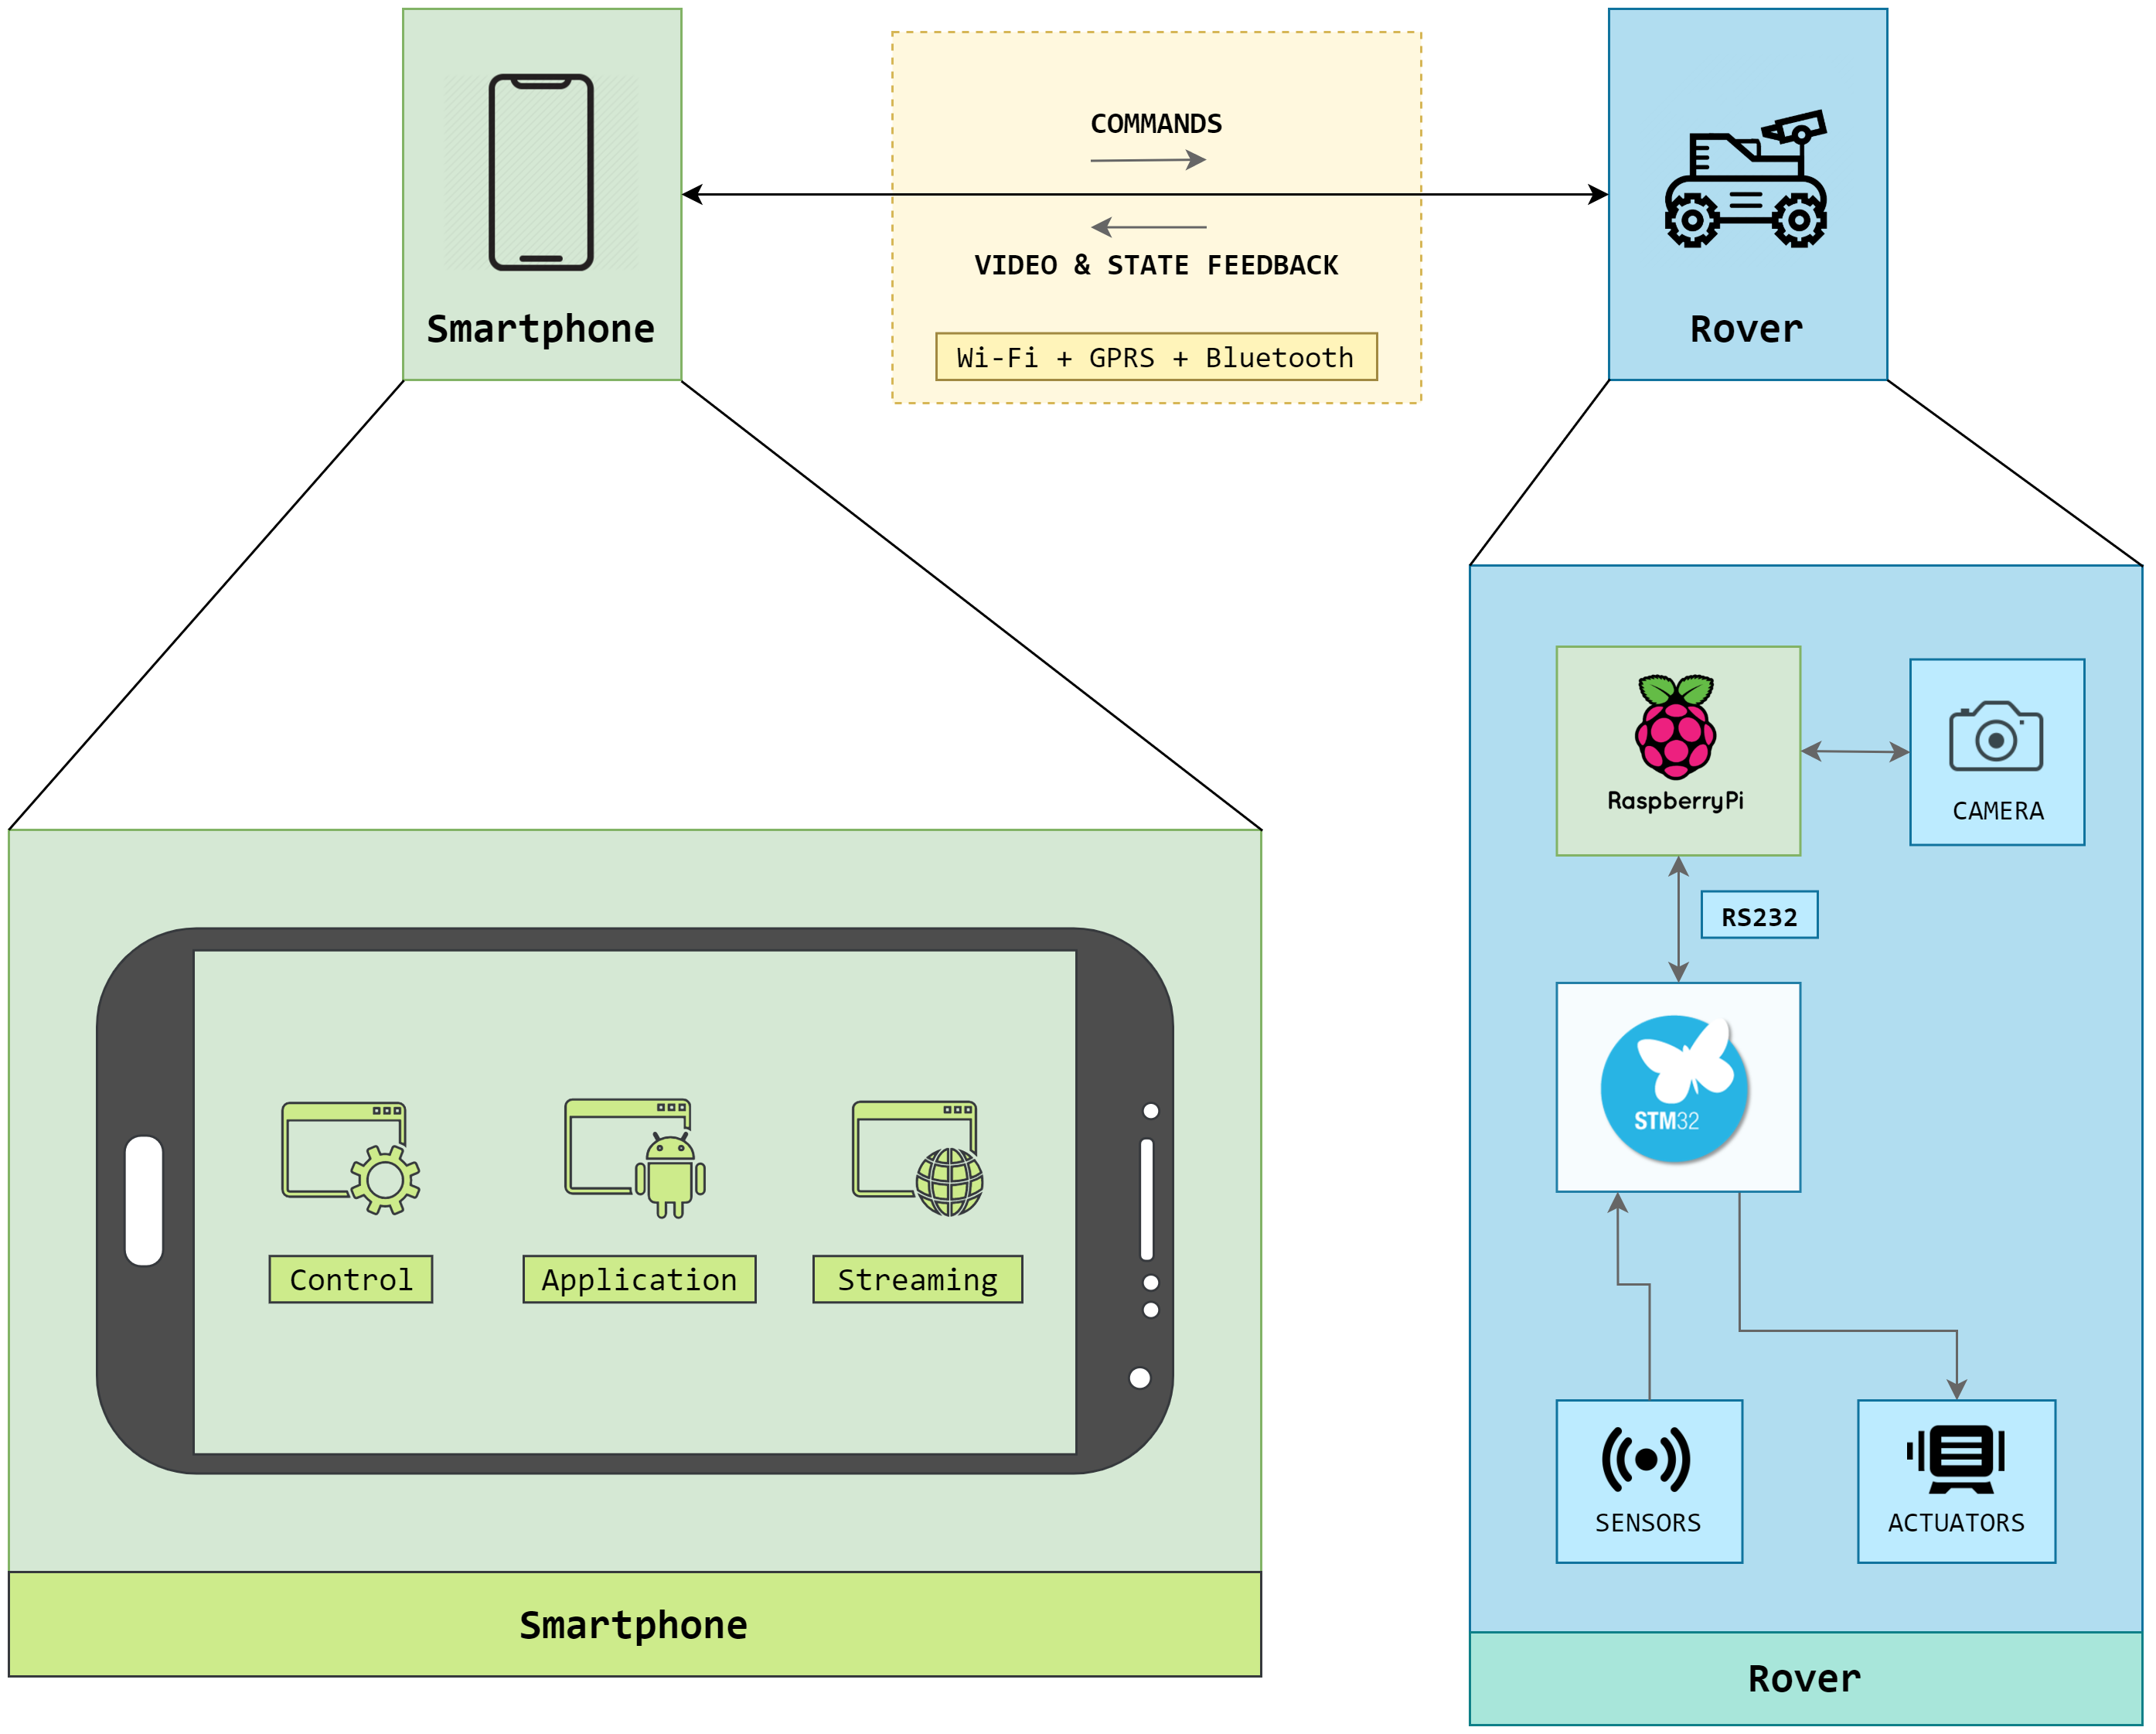
\includegraphics[width=1.0\textwidth]{./img/initial_design_diagram.png}
\caption{\label{fig:initial-design}Initial design: Block diagram view}
\end{figure}
\end{lstlisting}
\textbf{Result} (see Fig. \ref{fig:initial-design}):
\begin{figure}[!ht]
\centering
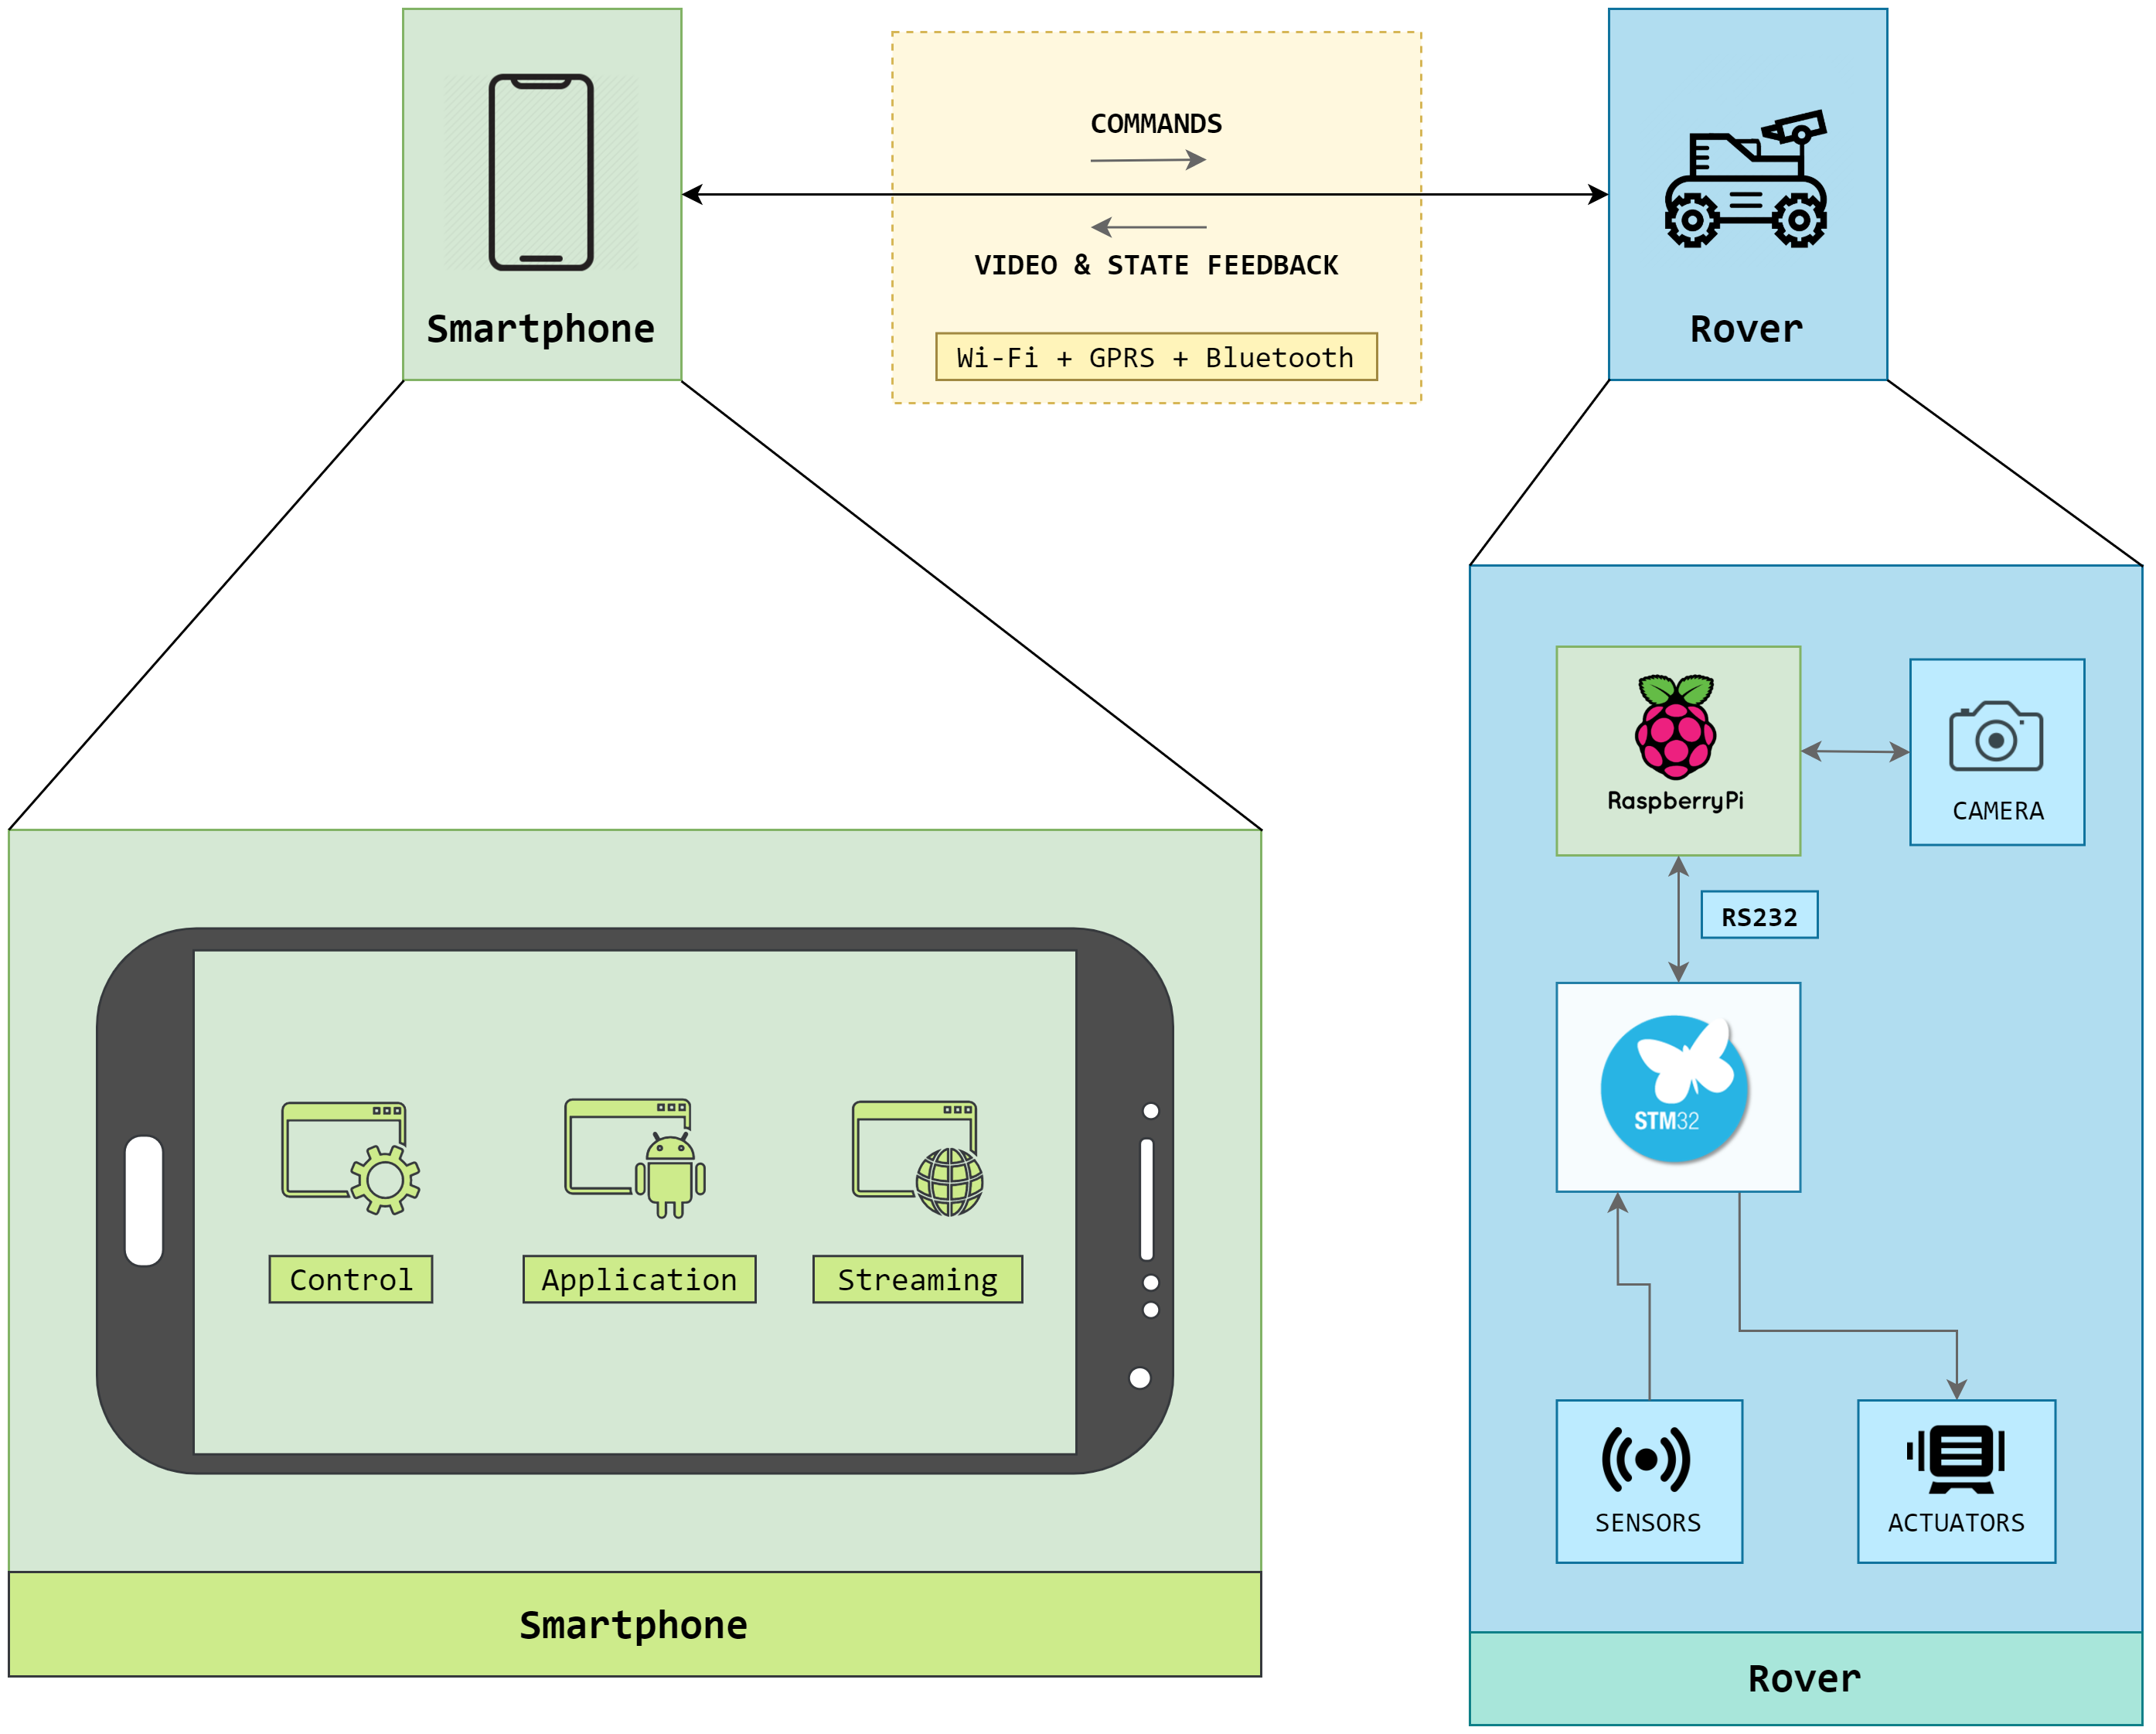
\includegraphics[width=1.0\textwidth]{./img/initial_design_diagram.png}
\caption{\label{fig:initial-design}Initial design: Block diagram view}
\end{figure}
\subsection{Tables}
\label{sec:orgd573a75}
\begin{enumerate}
\item Construction: Tables can be created using an online tool
(\url{https://www.tablesgenerator.com/}) and then copied, as illustrated in
\emph{Definition}
\item Definition: 
\lstset{language=[LaTeX]TeX,label= ,caption= ,captionpos=b,numbers=none}
\begin{lstlisting}
% Please add the following required packages to your document preamble:
% \usepackage[table,xcdraw]{xcolor}
\begin{table}[!hbt]
\centering
\caption{Specifications}%
\label{tab:specs-init}
%
\begin{tabular}{
>{\columncolor[HTML]{FFFFFF}}l 
>{\columncolor[HTML]{FFFFFF}}l 
>{\columncolor[HTML]{FFFFFF}}l }
\hline
		& Values     & Explanation                                                                                                  \\ \hline
Autonomy          & 4 h        & \begin{tabular}[c]{@{}l@{}}Time interval between battery fully \\ charged and safely discharged\end{tabular} \\ \hline
Speed Range  & 0.1 to 1 m/s    & \begin{tabular}[c]{@{}l@{}}Speed at which the car can operate\end{tabular}              \\ \hline
Frame Rate        & 60 fps     & \begin{tabular}[c]{@{}l@{}}Frequency at which independent still \\ images appear on the screen\end{tabular}  \\ \hline
Camera Range      & 20 m       & \begin{tabular}[c]{@{}l@{}}How far can the camera capture images\\ without loosing resolution\end{tabular}   \\ \hline
Camera resolution & 480p       & Amount of detail that the camera can capture                                                                 \\ \hline
Communication Range & 50 m & \begin{tabular}[c]{@{}l@{}}Maximum distance between the car and the\\ smarphone without losing connection\end{tabular} \\ \hline
speed Error    & 5 \%       & \begin{tabular}[c]{@{}l@{}}Maximum difference between desired \\ and real speed\end{tabular}              \\ \hline
Direction Error   & 5\%        & \begin{tabular}[c]{@{}l@{}}Maximum difference between desired\\  and real direction\end{tabular}             \\ \hline
Distance Error     & 5 \% & \begin{tabular}[c]{@{}l@{}}Maximum difference between desired\\ and real distance to the obstacle\end{tabular}         \\ \hline
Dimensions        & 20x12x5 cm & Dimensions of the car                                                                                        \\ \hline
Weight            & 0.5 kg     & Weight of the car                                                                                            \\ \hline
\end{tabular}
\end{table}
\end{lstlisting}
\item \textbf{Result}: Table \ref{tab:specs-init} lists the foreseen product
specifications.
\begin{table}[!hbt]
\centering
\caption{Specifications}%
\label{tab:specs-init}
%
\begin{tabular}{
>{\columncolor[HTML]{FFFFFF}}l 
>{\columncolor[HTML]{FFFFFF}}l 
>{\columncolor[HTML]{FFFFFF}}l }
\hline
		& Values     & Explanation                                                                                                  \\ \hline
Autonomy          & 4 h        & \begin{tabular}[c]{@{}l@{}}Time interval between battery fully \\ charged and safely discharged\end{tabular} \\ \hline
Speed Range  & 0.1 to 1 m/s    & \begin{tabular}[c]{@{}l@{}}Speed at which the car can operate\end{tabular}              \\ \hline
Frame Rate        & 60 fps     & \begin{tabular}[c]{@{}l@{}}Frequency at which independent still \\ images appear on the screen\end{tabular}  \\ \hline
Camera Range      & 20 m       & \begin{tabular}[c]{@{}l@{}}How far can the camera capture images\\ without loosing resolution\end{tabular}   \\ \hline
Camera resolution & 480p       & Amount of detail that the camera can capture                                                                 \\ \hline
Communication Range & 50 m & \begin{tabular}[c]{@{}l@{}}Maximum distance between the car and the\\ smarphone without losing connection\end{tabular} \\ \hline
speed Error    & 5 \%       & \begin{tabular}[c]{@{}l@{}}Maximum difference between desired \\ and real speed\end{tabular}              \\ \hline
Direction Error   & 5\%        & \begin{tabular}[c]{@{}l@{}}Maximum difference between desired\\  and real direction\end{tabular}             \\ \hline
Distance Error     & 5 \% & \begin{tabular}[c]{@{}l@{}}Maximum difference between desired\\ and real distance to the obstacle\end{tabular}         \\ \hline
Dimensions        & 20x12x5 cm & Dimensions of the car                                                                                        \\ \hline
Weight            & 0.5 kg     & Weight of the car                                                                                            \\ \hline
\end{tabular}
\end{table}
\end{enumerate}
\section{Referencing}
\label{sec:org4434181}
To reference the relevant items such as figures, tables, sections (chapter,
section, subsection), etc., one needs:
\begin{enumerate}
\item To label the item, using \texttt{\textbackslash{}label\{<item>:<item-name>\}}:
e.g. \texttt{\textbackslash{}label\{ch:analysis\}}
\item Then, one can reference it using: \texttt{\textbackslash{}ref\{<item>:<item-name>\}}:
e.g. Chapter\textasciitilde{}\ref{ch:analysis}
\end{enumerate}
\section{Bibliography}
\label{sec:orge62b455}
Bibliography management is composed of 2 parts:
\begin{enumerate}
\item A Bibliography database, generally a \texttt{.bib} file, located at
\texttt{./bib/dissert.bib} (see \href{file:///Users/zemiguel/Documents/Univ/MI\_Electro/Sem6/LPI2/PI/github/Deliverables/Final/bib/dissert.bib}{here})
\begin{itemize}
\item Example of Bibliography entry
\lstset{language=[LaTeX]TeX,label= ,caption= ,captionpos=b,numbers=none}
\begin{lstlisting}
@article{harashima1996mechatronics,
  title={Mechatronics-" What Is It, Why, and How?" An Editorial},
  author={Harashima, Fumio and Tomizuka, Masayoshi and Fukuda, Toshio},
  journal={IEEE/ASME Transactions on Mechatronics},
  volume={1},
  number={1},
  pages={1--4},
  year={1996},
  publisher={IEEE}
}
\end{lstlisting}
\item Bibliography entry can be created as:
\begin{itemize}
\item Search the topic at \url{https://scholar.google.pt/}.
\item Select the Export To Bibtex option
\item Copy to the \texttt{.bib} file
\end{itemize}
\end{itemize}
\item A citation, using \texttt{\textbackslash{}cite\{<bib-key>\}}, where \texttt{<bib-key>} is the key defined in
the \texttt{.bib} file. 
\begin{itemize}
\item For example: Mechatronics, was defined by Harashima
et. al=\textasciitilde{}\cite{harashima1996mechatronics}=
\end{itemize}
\end{enumerate}
\section{Enviroments}
\label{sec:org4102c27}
\subsection{Itemize}
\label{sec:org574551c}
\lstset{language=[LaTeX]TeX,label= ,caption= ,captionpos=b,numbers=none}
\begin{lstlisting}
\begin{itemize}
\item \textbf{Item 1}: this is an item
\item \textbf{Item 2}: this is another item
\end{itemize}
\end{lstlisting}
\textbf{Result}:
\begin{itemize}
\item \textbf{Item 1}: this is an item
\item \textbf{Item 2}: this is another item
\end{itemize}

\subsection{Enumerate}
\label{sec:org9d11cf3}
\lstset{language=[LaTeX]TeX,label= ,caption= ,captionpos=b,numbers=none}
\begin{lstlisting}
\begin{enumerate}
\item \textbf{Item 1}: this is an enumerated item
\item \textbf{Item 2}: this is another enumerated item
\end{enumerate}
\end{lstlisting}
\textbf{Result}:
\begin{enumerate}
\item \textbf{Item 1}: this is an enumerated item
\item \textbf{Item 2}: this is another enumerated item
\end{enumerate}
\section{Glossary}
\label{sec:org8845f59}
Glossaries are useful to input \uline{acronyms} and \uline{symbols}.
\begin{itemize}
\item Acronyms: common use words, often abbreviated.
\item Symbols: mathematical/physical symbols that usually require some brief
description and the relevant units.
\end{itemize}

Glossary management is composed of 3 parts:
\begin{enumerate}
\item A Glossary database 
\begin{itemize}
\item Acronyms: \texttt{./sec/acronyms.tex}
\item Symbols: \texttt{./sec/symbols.tex}
\end{itemize}
\item A reference using \texttt{\textbackslash{}gls\{<gls-key>\}}, where \texttt{<gls-key>} is the key defined in
the glossary database file.
\item An external utility that manages the glossary entry items addition and
referencing (no need to worry about this, the makefile will handle it).
\end{enumerate}
\subsection{Acronyms}
\label{sec:orgc5e2914}
\begin{itemize}
\item Definition (\texttt{./sec/acronyms.tex}):
\lstset{language=[LaTeX]TeX,label= ,caption= ,captionpos=b,numbers=none}
\begin{lstlisting}
\newacronym{sls}{SLS}{Selective Laser Sintering}
\newacronym{slm}{SLM}{Selective Laser Melting}
\end{lstlisting}
\item Usage: These are two acronyms used together: \texttt{\textbackslash{}gls\{sls\}/\textbackslash{}gls\{slm\}} technology.
\end{itemize}

\subsection{Symbols}
\label{sec:orgd66ae0b}
\begin{itemize}
\item Definition (\texttt{./sec/symbols.tex}):
\lstset{language=[LaTeX]TeX,label= ,caption= ,captionpos=b,numbers=none}
\begin{lstlisting}
\newglossaryentry{omega}
{
    name={\ensuremath{\omega}},
    description={angular velocity},
    sort=omega,
    symbol={\ensuremath{\omega}},
    unit={\si{rad/s}}
}
\end{lstlisting}
\item Usage: this is \texttt{\textbackslash{}gls\{omega\}}.
\end{itemize}

\section{Listings}
\label{sec:org52673a7}
\begin{itemize}
\item Styling: Listings can be formatted using different styles, as presented in
\texttt{./sty/listing.sty} for any programming/markup language required.
\begin{itemize}
\item Example: C
\lstset{language=[LaTeX]TeX,label= ,caption= ,captionpos=b,numbers=none}
\begin{lstlisting}
\lstdefinestyle{customc}{
belowcaptionskip=1\baselineskip,
breaklines=true,
%frame=L,%lines, whole
xleftmargin=\parindent,
language=C,
showstringspaces=false,
basicstyle=\scriptsize\ttfamily,
keywordstyle=\bfseries\color{green!40!black},
commentstyle=\itshape\color{purple!40!black},
identifierstyle=\color{blue},
stringstyle=\color{orange},
numberstyle={\tiny},
numbers=left,
numberblanklines=false,
stepnumber=5,
backgroundcolor=\color{yellow!10}, 
frame=tlb
}
\end{lstlisting}
\end{itemize}
\item Usage: Listings can be inputted using the desired style as below. It includes
a caption, a label, a style, and a file path:
\lstset{language=[LaTeX]TeX,label= ,caption= ,captionpos=b,numbers=none}
\begin{lstlisting}
\lstinputlisting[language=C++, caption={Thread Serial Rx handler},label=lst:threadSerialRx,
style=customc]{./listing/threadSerialRx.cpp}%
\end{lstlisting}
\item Result:
\end{itemize}
\lstset{language=C,label= ,caption= ,captionpos=b,numbers=none,style=customc}
\begin{lstlisting}
UINT MMSLSDlg::ThreadSerialRx(LPVOID param)
{
    /* Wait for 1st connection to serial port: OnConnect */
    ::WaitForSingleObject( EvSerial.m_hObject , INFINITE); 
    tstring szData;
    CDemoEzdDlg *dlg = (CDemoEzdDlg *)param;

    while(1)
    ;

    return 0;
}
\end{lstlisting}
\section{PDF inclusion}
\label{sec:orgd6f8882}
\begin{itemize}
\item Include all pages from \texttt{anexo3-license}. Be careful of file path. It's
relative to the main file.
\lstset{language=[LaTeX]TeX,label= ,caption= ,captionpos=b,numbers=none}
\begin{lstlisting}

\includepdf[pages=-]{anexo3-license}
\end{lstlisting}
\end{itemize}
\section{Appendices}
\label{sec:org8624020}
Appendices can be added in the appropriate section (\texttt{./tex/Append/}):
\begin{itemize}
\item as text: with figures, tables, etc.
\item included as PDF
\end{itemize}
\end{document}